\documentclass{beamer}
\usepackage[utf8]{inputenc}
\usepackage[spanish,es-tabla]{babel}
\usepackage{graphicx}
\usepackage{movie15}
\graphicspath{ {imagenes/} }

\usetheme{Berlin}

\title{Interacción Humano Computador}

\author{Christofer Fabián Chávez Carazas}

\institute[Universidad Nacional de San Agustín] 


\date{\today}

\subject{IHC}
\AtBeginSubsection[]
{
  \begin{frame}<beamer>{Outline}
    \tableofcontents[currentsection,currentsubsection]
  \end{frame}
}

\begin{document}

\begin{frame}
  \titlepage
\end{frame}

\begin{frame}
\begin{block}{1. Describa el proceso de interacción y sus componentes}
El proceso de Interacción es el intercambio de acciones entre uno o más entidades con la intención de comunicarse.
\begin{itemize}
    \item Directa
    \item Indirecta
\end{itemize}

\includegraphics[scale = 0.45]{1.jpg}
\vspace{0.5}

\includegraphics[scale = 0.3]{2.jpg}
\end{block}
\end{frame}

\begin{frame}
\begin{block}{2. Describa lo que es la comunicación y sus componentes}
La Comunicación es un proceso de intercambio de información, en el que un emisor transmite a un receptor algo a través de un canal esperando que, posteriormente, se produzca una respuesta de dicho receptor, en un contexto determinado.
\begin{center}

\includegraphics[scale = 0.1]{3.png}
\end{center}
\end{block}
\end{frame}

\begin{frame}
\begin{block}{3. Explique por qué es importante el estudio de la interacción humano-computadora}
Por la importancia de saber sobre la comunicación entre el humano y el computador que hoy en día es casi indispensable. Una mala interacción con la computadora significa perdidas para el usuario (timepo) y para los desarrolladores (dinero).
\begin{center}
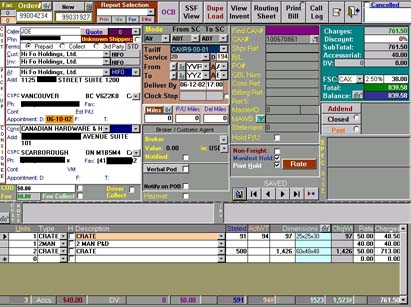
\includegraphics[scale = 0.4]{3_1.jpg}
\end{center}
\end{block}
\end{frame}

\begin{frame}
\begin{block}{4. Defina lo que es una interfaz de usuario}
La interfaz de usuario es el medio con que el usuario puede comunicarse con una máquina, equipo, computadora o dispositivo, y comprende todos los puntos de contacto entre el usuario y el computador.
\begin{center}
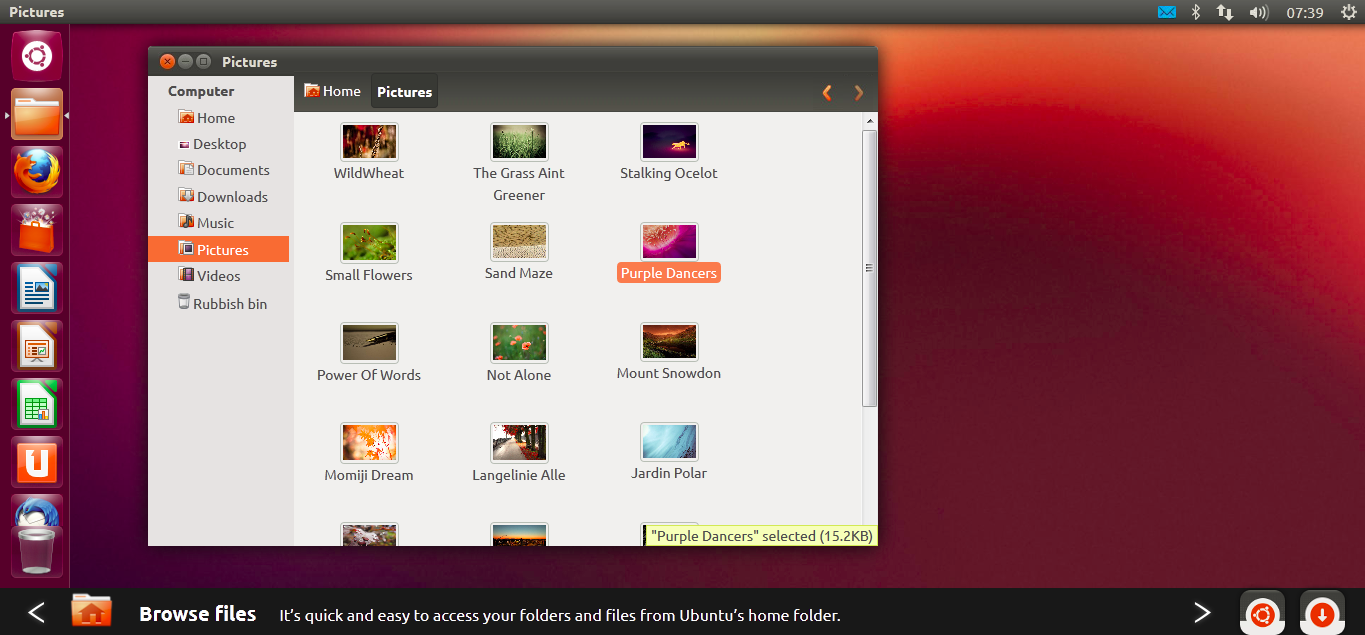
\includegraphics[scale = 0.2]{4.png}
\end{center}
\end{block}
\end{frame}

\begin{frame}
\begin{block}{5. Describa lo que es el Diseño Centrado en el Usuario (UCD) y diga cuales son los tres pilares que los sustentan}
El Diseño Centrado en el Usuario es una filosofía de diseño que tiene por objetivo la creación de productos que resuelvan necesidades concretas de sus usuarios finales, consiguiendo la mayor satisfacción y mejor experiencia de uso posible con el mínimo esfuerzo de su parte.
\begin{itemize}
    \item La Ingeniería del Software
    \item El Prototipado
    \item La Evaluación
\end{itemize}
\end{block}
\end{frame}

\begin{frame}
  \begin{center}
  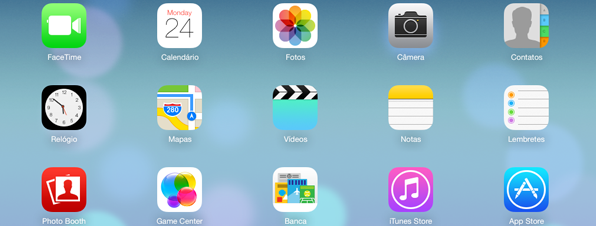
\includegraphics[scale = 0.5]{4_1.png}
  \end{center}
\end{frame}



\begin{frame}
\begin{block}{6. Mencione cinco de los seis principios del diseño centrado en el usuario}
\begin{itemize}
    \item El proceso de desarrollo debe estar basado en el entendimiento del usuario.
    \item El usuario debe participar en todo el proceso de desarrollo y diseño.
    \item El diseño es dirigido y refinado a través de la evaluación centrada en el usuario.
    \item El diseño contempla toda la experiencia del usuario en el sistema
    \item El equipo de desarrollo incluye perspectivas y habilidades multi-disciplinares.
\end{itemize}
\end{block}
\end{frame}

\begin{frame}
\begin{block}{7. Mencione algunos de los factores humanos que afectan el proceso de interacción}
Deficiencias físicas o cognitivas, Factores culturales o contextuales del entorno, factores
humanos de los usuarios objetivo, factores etnográficos, factores dinámicos del entorno
físico, etc.
\begin{center}
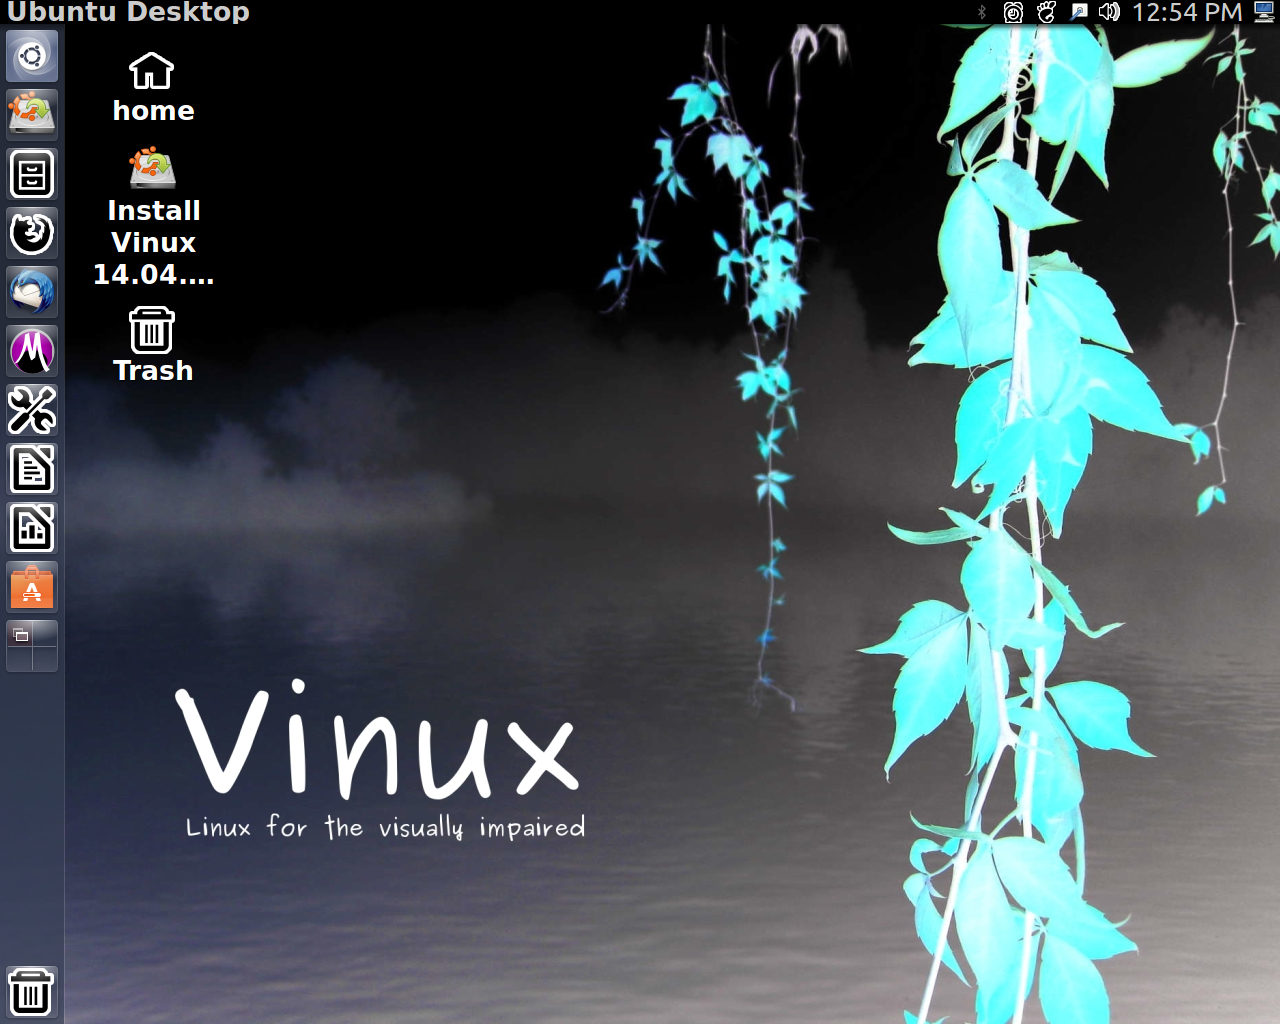
\includegraphics[scale = 0.1]{5.png}
\vspace{0.5}
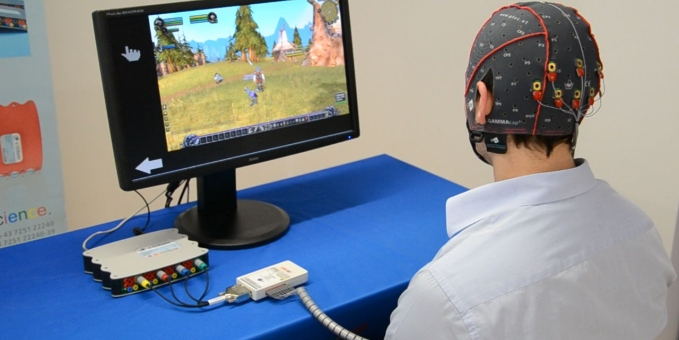
\includegraphics[scale = 0.25]{5_1.jpg}
\end{center}
\end{block}
\end{frame}

\begin{frame}
\begin{block}{8. Mencione las fases del Diseño Centrado en el Usuario:}
\begin{center}
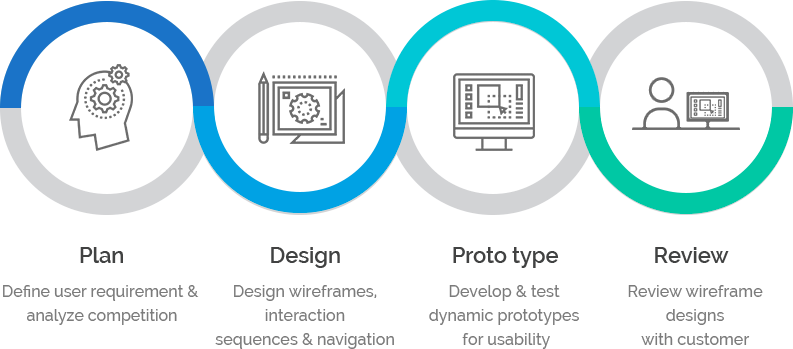
\includegraphics[scale = 0.35]{6.png}
\end{center}
\end{block}
\end{frame}

\begin{frame}
\begin{block}{9. Mencione tres metodologías de desarrollo que contemplen o integren aspectos del
Diseño Centrado en el Usuario en sus fases de desarrollo.}
\begin{itemize}
    \item MPIu+a: Modelo de Proceso de la Ingeniería de la usabilidad y de la accesibilidad propone un enfoque donde se aplican aspectos del DCU a las fases del desarrollo del software.
    \item ISO 13407: Human-centred design processes for interactive systems constituye un marca que sirve de guía para conseguir el desarrollo de sistemas interactivos usables incorporando el DUC durante el ciclo de vida del desarrollo.
    \item RACED, Modelo Centrado en el Usuario para el Desarrollo Ágil de Videojuegos Casuales en Dispositivos Móviles.
\end{itemize}
\end{block}
\end{frame}


\begin{frame}
\begin{block}{10. ¿A qué se refiere el concepto de paradigma de interacción?}
Son los modelos de los que se derivan todos los sistemas de interacción.
\end{block}
\begin{block}{11. Describir cuatro paradigmas de interacción}
\begin{itemize}
    \item La computadora de escritorio.
    \item Computación ubícua.
    \item Realidad virtual.
    \item Realidad aumentada.
\end{itemize}
\end{block}
\end{frame}

\begin{frame}

\begin{center}
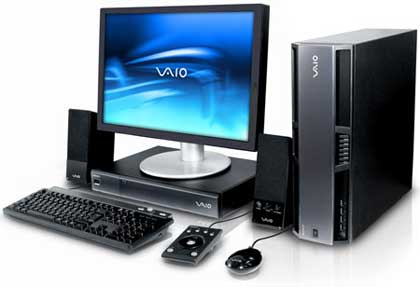
\includegraphics[scale = 0.25]{7_1.jpeg}
\vspace{0.5}
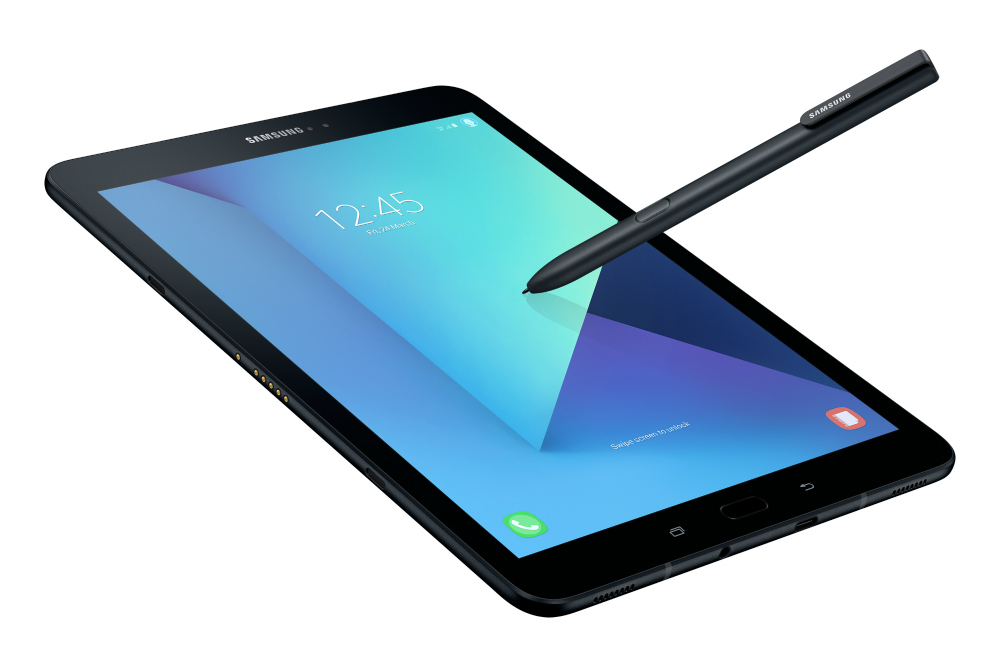
\includegraphics[scale = 0.1]{7_2.jpg} \\
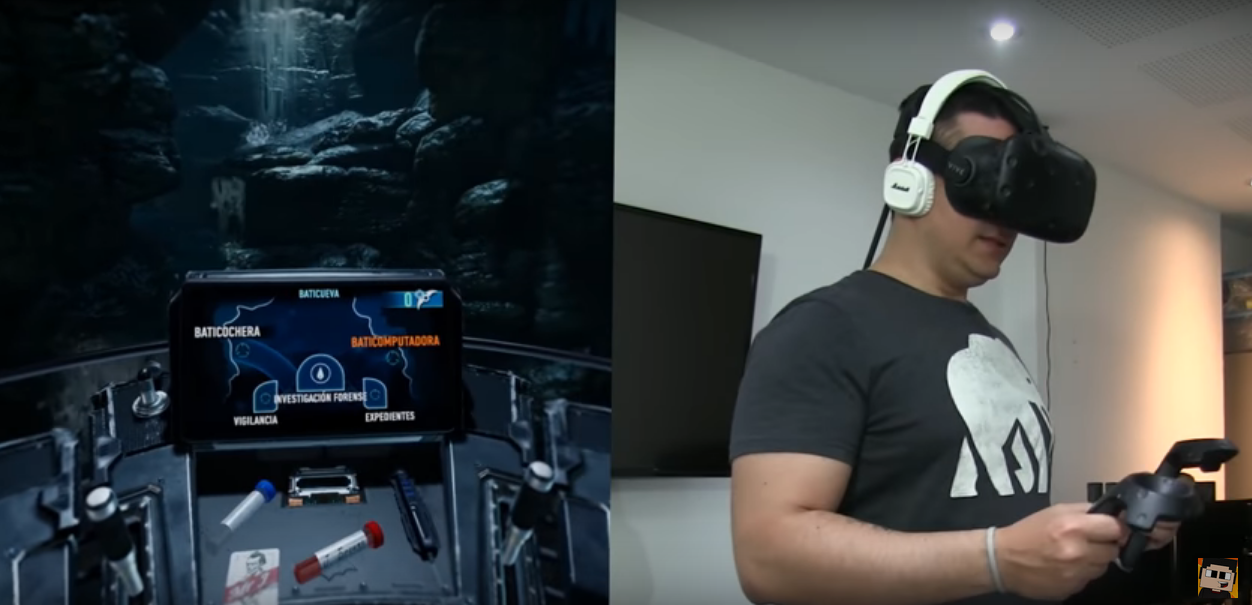
\includegraphics[scale = 0.2]{7.png}
\end{center}
\end{frame}

\begin{frame}
\begin{center} 
 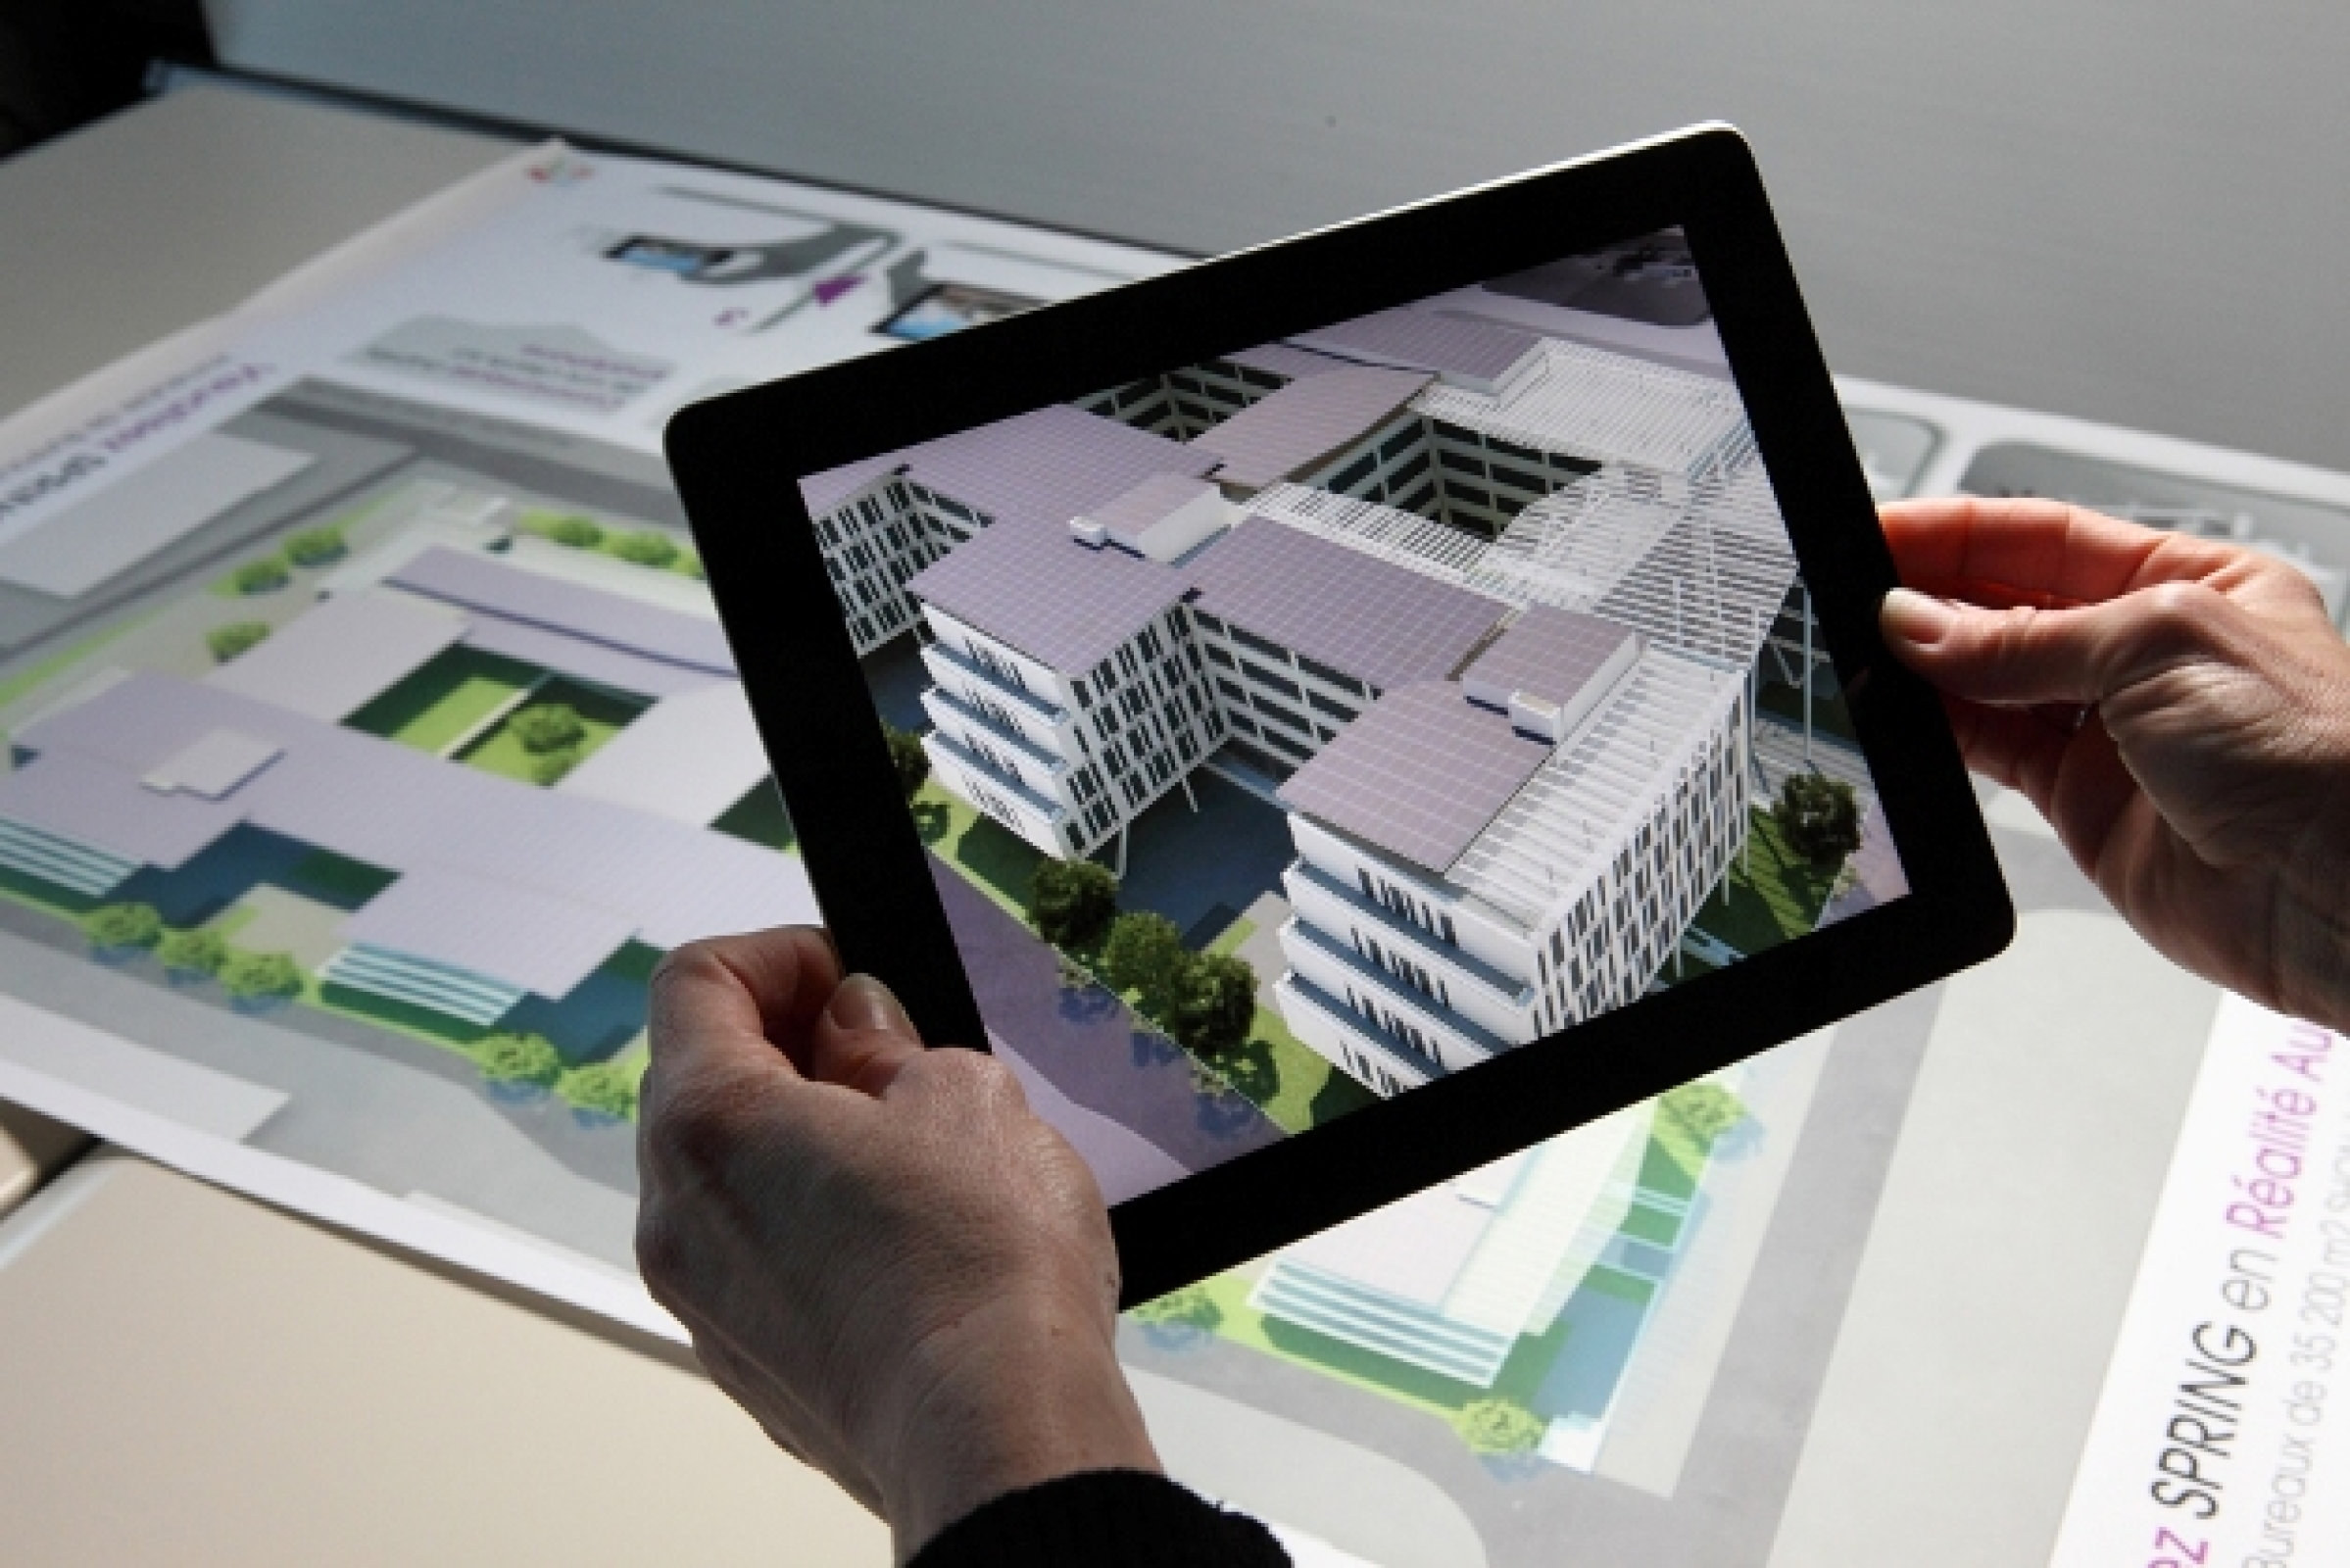
\includegraphics[scale = 0.4]{7_3.jpg}
\end{center}

\end{frame}


\begin{frame}
\begin{block}{12. Explicar los prototipos en el Diseño Centrado en el Usuario}
Los prototipos son documentos, diseños o sistemas que simulan o tienen implementadas partes del sistema final.
\end{block}
\begin{block}{13. Mencione 4 características de los prototipos.}
\begin{itemize}
    \item Son operativos.
    \item Tienen un tiempo de vida corto.
    \item Pueden servir para diferentes objetivos.
    \item Pueden ser construidos rápida y eficientemente.
\end{itemize}
\end{block}
\end{frame}

\begin{frame}
\begin{center}
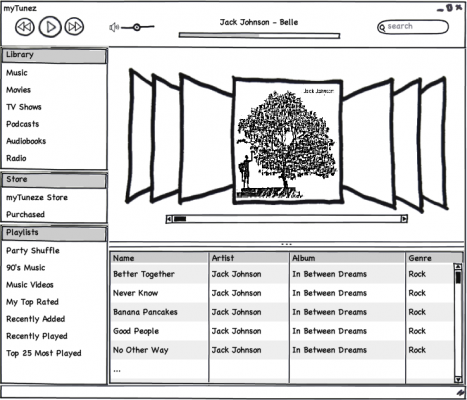
\includegraphics[scale = 0.4]{8.png}
\end{center}
\end{frame}

\begin{frame}
\begin{block}{14. Describa lo que es un Escenario en el desarrollo de prototipos y cual es su utilidad}
Un escenario es “una historia de ficción con representación de personajes, sucesos, productos y entornos”. Ayuda al diseñador a explorar ideas y las ramificaciones de decisiones de diseño en situaciones concretas.
\end{block}
\begin{block}{15. ¿Cuál es el objetivo del diseño de interfaces de usuario?}
Crear una interfaz clara y limpia que el usuario pueda entender y usar con facilidad.
\end{block}
\end{frame}

\begin{frame}
\begin{center}
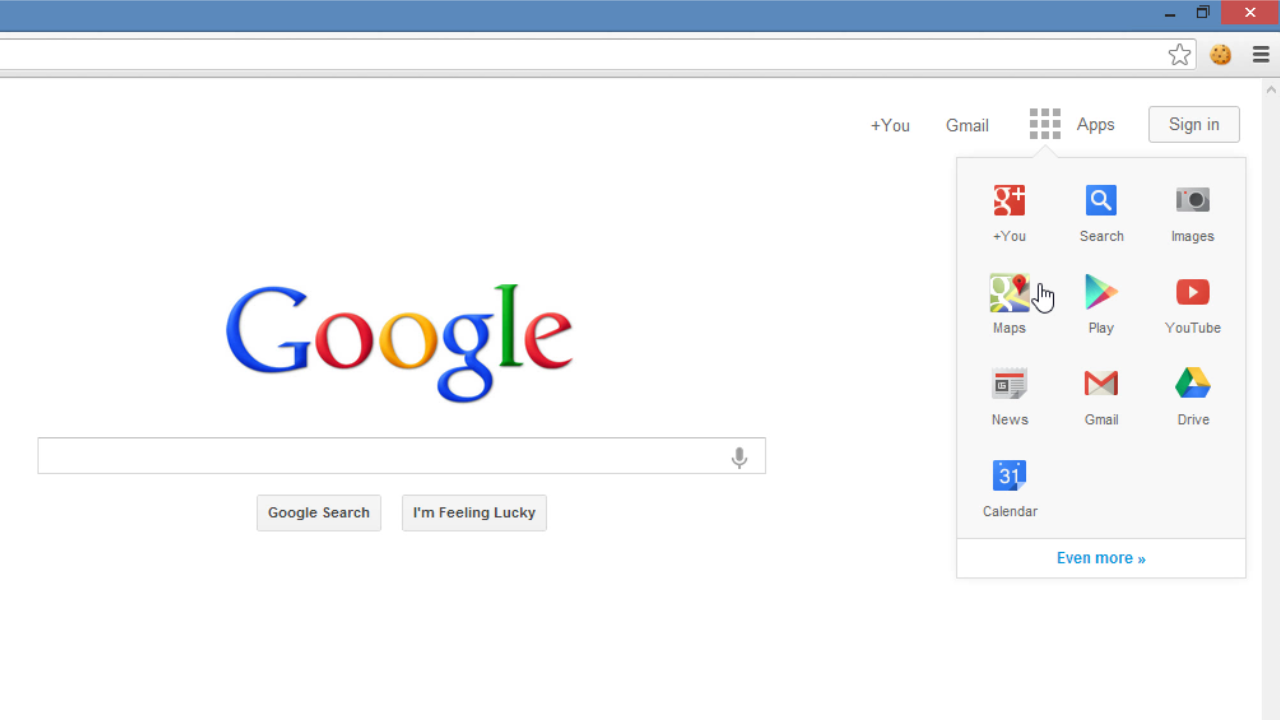
\includegraphics[scale = 0.2]{9.png}
\end{center}
\end{frame}

\begin{frame}
\begin{block}{16. Describir los siguientes 9 elementos de la imagen.}
El punto: El punto es la señal más sencilla que puede utilizar un comunicador en el plano de la comunicación visual. Por ejemplo, un ritmo de composición.
\begin{center}
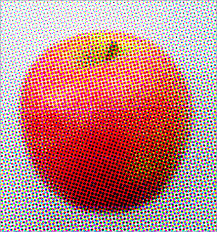
\includegraphics[scale = 0.5]{10.jpeg}
\end{center}
\end{block}
\end{frame}

\begin{frame}
\begin{block}{}
\begin{itemize}
    \item La línea: Puede definirse como una sucesión ininterrumpida de puntos. En tanto más unidos se hallen más concreción proporcionan a la línea.
    \item La forma: Cuando la linea se cierra sobre si misma describe un contorno determinando una tensión entre el espacio creado y sus límites. Los contornos pueden ser estáticos o dinámicos dependiendo del uso que se les dé o de las diferentes direcciones que éste adopte.
\end{itemize}
\end{block}
\end{frame}

\begin{frame}
\begin{block}{}
\begin{itemize}
    \item La luz: Elemento fundamental en la composición de una imagen. Se usa para expresar sentimientos o emociones, crear una atmósfera poética, diferenciar distintos aspectos de una representación, y resaltar la profundidad de los ambientes cerrados y de los espacios abiertos.
    \item El color: El color es el efecto de las radiaciones visibles que forman parte del espectro electromagnético.
    \item El tamaño: Por tamaño entendemos la relación entre la imagen reproducida y el espacio que ocupa en el soporte. El tamaño condiciona de forma poderosa la sensación del espectador ante una imagen.
\end{itemize}
\end{block}
\end{frame}


\begin{frame}
\begin{center}
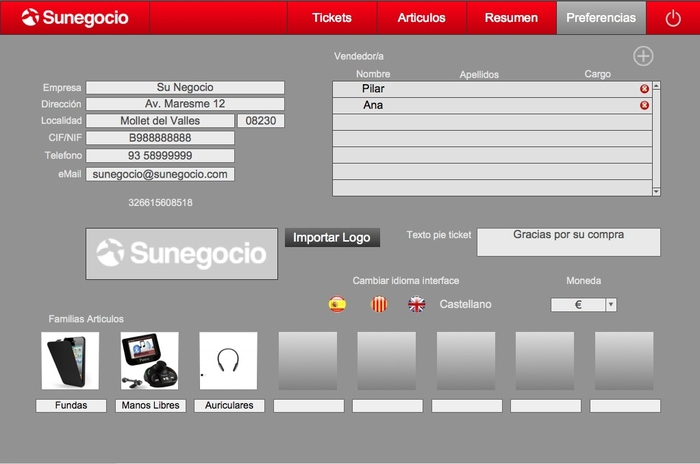
\includegraphics[scale = 0.4]{11.jpg}
\end{center}
\end{frame}


\begin{frame}
\begin{block}{}
\begin{itemize}
 \item El formato: Constituyen las dimensiones de la imagen: anchura y altura y su relación. El formato determina el encuadre y es el punto de partida de la composición a través de las proporciones y la orientación. Existen formatos rectangulares, circulares, elípticos y poligonales.   
 \item La composición: Es la disposición equilibrada de los elementos de la imagen que se ordenan para expresar sensaciones favorables en un espacio determinado. La distribución de estos elementos debe realizarse en función de una estructura interna que tenga una significación clara o una intención coincidente con el mensaje que se quiera transmitir.
\end{itemize}
\end{block}
\end{frame}


\begin{frame}
\begin{block}{17. Describa cuatro técnicas de diseño gráfico de interfaces de usuario}
\begin{itemize}
 \item Disposición: Cómo se colocan las cosas en la pantalla. Permite dar más importancia a ciertas cosas. El orden de lectura es importante y varía según la cultura.

\item Énfasis: Los elementos realzados se ven antes y se perciben como más importantes. Para enfatizar se usa la posición, el color y los atributos del texto.

\item Foco: El punto focal es el centro de atención, el punto que normalmente se ve antes. Se puede utilizar para dirigir al usuario a la información deseada. 

\item Alineación: Ayuda a conseguir equilibrio, armonía, unidad y modularidad. Una alineación exacta y consistente es la manera más fácil de mejorar la estética de la interfaz. 
\end{itemize}
\end{block}
\end{frame}
 
\begin{frame}
 \begin{center}
 
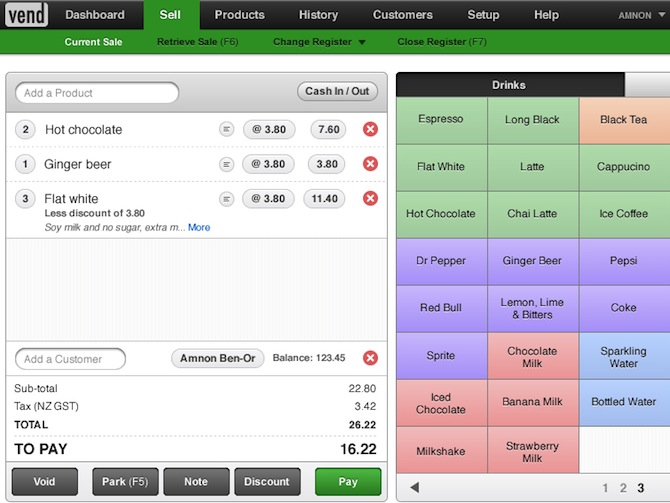
\includegraphics[scale = 0.4]{11.jpeg}
\end{center}
\end{frame}



\begin{frame}
\begin{block}{18. Defina lo que es un software internacionalizado}
Es un producto de software que está preparado para ser utilizado fuera de la región o país
donde fue creado. Su objetivo es hacer llegar el producto a mercados internacionales y el
problema que enfrenta es el de ajustar sus interfaces de usuario para las usuarios en los
diferentes destinos.
\begin{center}
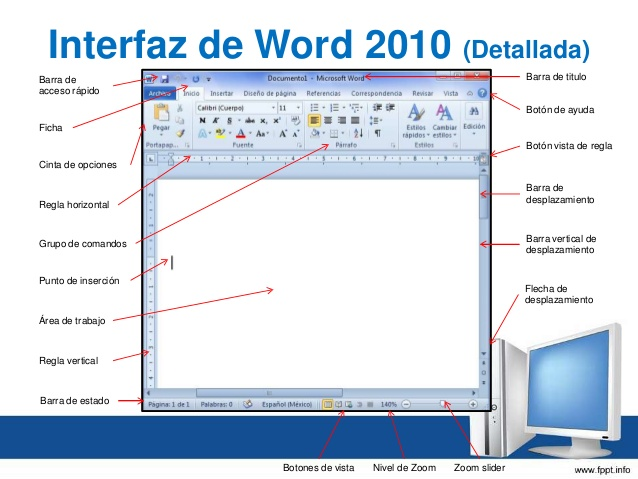
\includegraphics[scale = 0.25]{12.png}
\end{center}
\end{block}
\end{frame}


\begin{frame}
\begin{block}{19. Mencione tres ventajas de la internacionalización en un software}
\begin{itemize}
 \item El mismo software funciona para varios tipos de usuarios identificados por su cultura, nacionalidad u otras características generales.
 \item El mercado al que accede es mayor.
 \item El mantenimiento del software y la inclusión de nuevas regiones o localizaciones es menos costosa.
\end{itemize}
\end{block}
\end{frame}


\begin{frame}
\begin{block}{20. Mencione 5 elementos a considerar en el proceso de internacionalización de un software
tomando en cuenta aspectos culturales de los usuarios}
\begin{itemize}
 \item El idioma
 \item El audio (voz)
 \item Formatos de monedas, fechas y números
 \item Calendarios
 \item Medidas
\end{itemize}
\end{block}
\end{frame}

\begin{frame}
 \begin{center}
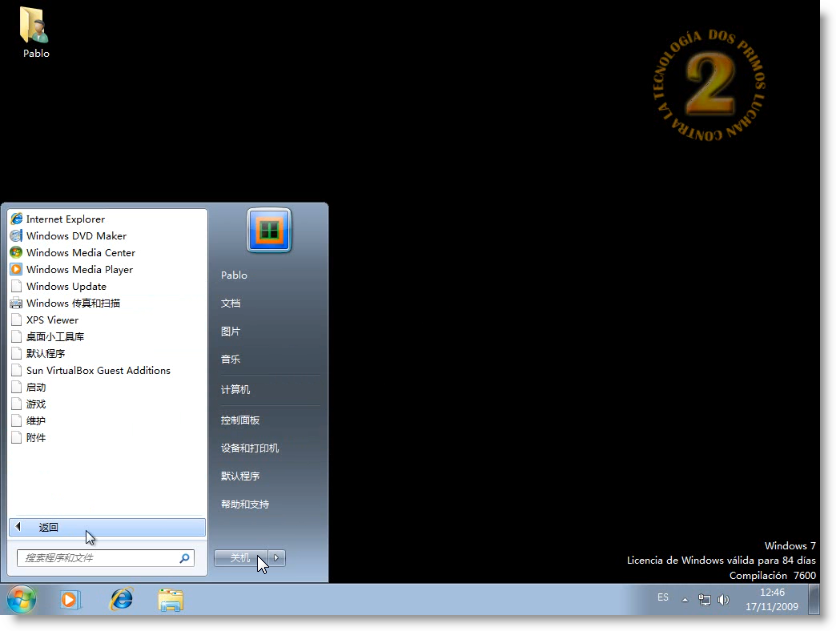
\includegraphics[scale = 0.4]{13.png}
\end{center}
\end{frame}

\begin{frame}
\begin{block}{21. Describa tres objetivos del estudio de la accesibilidad para el desarrollo de sistemas interactivos}
\begin{itemize}
 \item Promover la concienciación de los diseñadores y programadores de interfaces de usuario acerca de la necesidad del diseño universal.
 \item Motivar a la utilización de técnicas de usabilidad teniendo también en cuenta a usuarios
con discapacidades.
 \item Conocer los diversos tipos de discapacidades y algunas de las soluciones disponibles
más extendidas.
\end{itemize}
\end{block}
\end{frame}

\end{document}


